\newpage
\section{Classification of Self-Adaptive Systems}
\label{ch:SASClassification}

% TODO:
% - Shortly cover how SAS are classified:
%     - Krupitzer et al
%     - "Towards a taxonomy ..."
% - Which parts can be optimized?
% - Which parts cant be optimized/are a design decision?
% - Current landscape of OA
%     - mostly ML

% \begin{itemize}
%     \item How Self-Adaptive Systems are classified.
%     \item Which parts of Self-Adaptive Systems can be optimized or are important for optimization.
%     \item An overview of current optimization approaches for Self-Adaptive Systems.
% \end{itemize}

% \paragraph*{Literature for this section:} \begin{itemize}
%     \item "A survey on engineering approaches for self-adaptive systems" \cite{SurveyOnEngineeringApproaches}
%     \item "Towards a Taxonomy for the Evaluation of Self-* Software" \cite{TaxonomyOfSelfSoftware}
%     \item "Dissecting Self-* Properties" \cite{DissectingSelfProperties}
%     \item "Self-Adaptive Software: Landscape and Research Challenges" \cite{LandscapeAndResearchChallenges}
%     \item "The Application of Machine Learning in Self-Adaptive Systems: A Systematic Literature Review" \cite{ApplicationOfMachineLearning}
%     \item "Comparison of Approaches for Self-Improvement in Self-Adaptive Systems" \cite{ComparisonOfSelfImprovement}
% \end{itemize}

% TODO: How are SAS classified
There are different approaches on how to classify and describe \acrlong{sas},
which all focus on different usages, like:
% TODO: Add usages
\begin{itemize}
    % TODO: Z notation reference?
    \item FORMS from Weyns et al., 2012\cite*{FORMS} which is a formal reference model for describing \acrlong{sas} using Z notation.
    \item Krupitzer's et al., 2015\cite*{SurveyOnEngineeringApproaches} taxonomy for \acrlong{sas}
    \item Raibulet's, 2018\cite*{TaxonomyOfSelfSoftware} taxonomy for self-* properties
\end{itemize} 
In this paper Krupitzer's et al., 2015\cite*{SurveyOnEngineeringApproaches} taxonomy for \acrlong{sas} will be used to classify \acrshort{sas}.

\begin{figure}[t]
    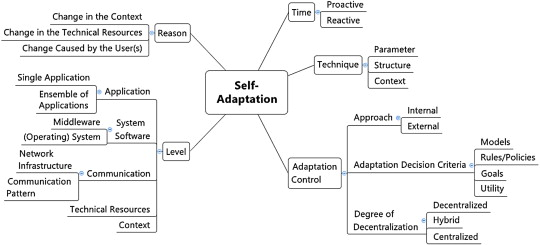
\includegraphics[width=\textwidth]{images/KrupitzerTaxonomy.jpg}
    \caption{Taxonomy for \acrlong{sas} by Krupitzer et al., 2015\cite*{SurveyOnEngineeringApproaches}}
    \label{fig:KrupitzerTaxonomy}
\end{figure}
The taxonomy in \figurename{\ref{fig:KrupitzerTaxonomy}} 
is based upon the 5W+1H questions by Salehie and Tahvildari, 2009\cite*{LandscapeAndResearchChallenges}.
These questions are: Where, When, What, Why, Who and How.
The question of who is responsible for an adaptation is trivially answered by the software itself.
For each of the remaining questions Krupitzer's et al., 2015\cite*{SurveyOnEngineeringApproaches} taxonomy offers a dimension:

% TODO: Which parts can be optimized

% TODO: Which parts cant be optimized/are a design descision

% TODO: Current landscape